\documentclass{article}

% Language setting
% Replace `english' with e.g. `spanish' to change the document language
\usepackage{biblatex} %Imports biblatex package
\addbibresource{../Lab2/refs.bib}
\usepackage{enumitem}
\usepackage[english]{babel}
\usepackage{array}
\usepackage{amsmath}
\usepackage{pythonhighlight}
\usepackage{multirow}
\newcolumntype{P}[1]{>{\centering\arraybackslash}p{#1}}
\newcolumntype{M}[1]{>{\centering\arraybackslash}m{#1}}

% Set page size and margins
% Replace `letterpaper' with `a4paper' for UK/EU standard size
\usepackage[letterpaper,top=2cm,bottom=2cm,left=3cm,right=3cm,marginparwidth=1.75cm]{geometry}

\usepackage{amsmath}
\usepackage{graphicx}
\usepackage[colorlinks=true, allcolors=blue]{hyperref}
\usepackage{setspace}
\usepackage{booktabs}
\usepackage[T1]{fontenc}
\usepackage{longtable}
\doublespacing

\begin{document}
\newcommand{\Fig}[3]{\begin{figure}[!h!]\centering\includegraphics[width=0.5\linewidth]{#1}\caption{#2}\label{#3}\end{figure}}
\begin{titlepage}

\centering
\scshape
\vspace{\baselineskip}

%
\rule{\textwidth}{1.6pt}\vspace*{-\baselineskip}\vspace*{2pt}
\rule{\textwidth}{0.4pt}

{\Huge \textbf{\textsc{ Cold Work and Annealing \\
\vspace{15pt}}}}

\rule{\textwidth}{0.4pt}\vspace*{-\baselineskip}\vspace{3.2pt}
\rule{\textwidth}{1.6pt}\vspace{6pt}
\centerline{\textit{University of Illinois at Urbana-Champaign}} 
\centerline{\textit{Department of Nuclear, Plasma, and Radiological Engineering}}
\vspace{1.5\baselineskip}


\large \centerline{\textbf{Author:} Nathan Glaser}
\large \centerline{\textbf{Net-ID:} nglaser3}
\quad

\vfill
\large \centerline{October 2, 2024}
%
\pagenumbering{gobble}
\end{titlepage}

\tableofcontents
\newpage
\pagenumbering{arabic}
 
\section{Abstract}

\section{Introduction}

\section{Theoretical Models}

\section{Experimental Methods}

\section{Results}
To begin, we plotted the cooling curve for pure Tin and 90\% Bismuth by weight fraction. The liquidus is marked with a black dotted line, on the temporal axis for clarity, and the solidus for the latter figure is marked with a maroon dotted line, again on the temporal axis for clarity. The true liquidus and solidus points are the intercepts between the curve and their respective dotted lines. 

\begin{figure}
    \centering
    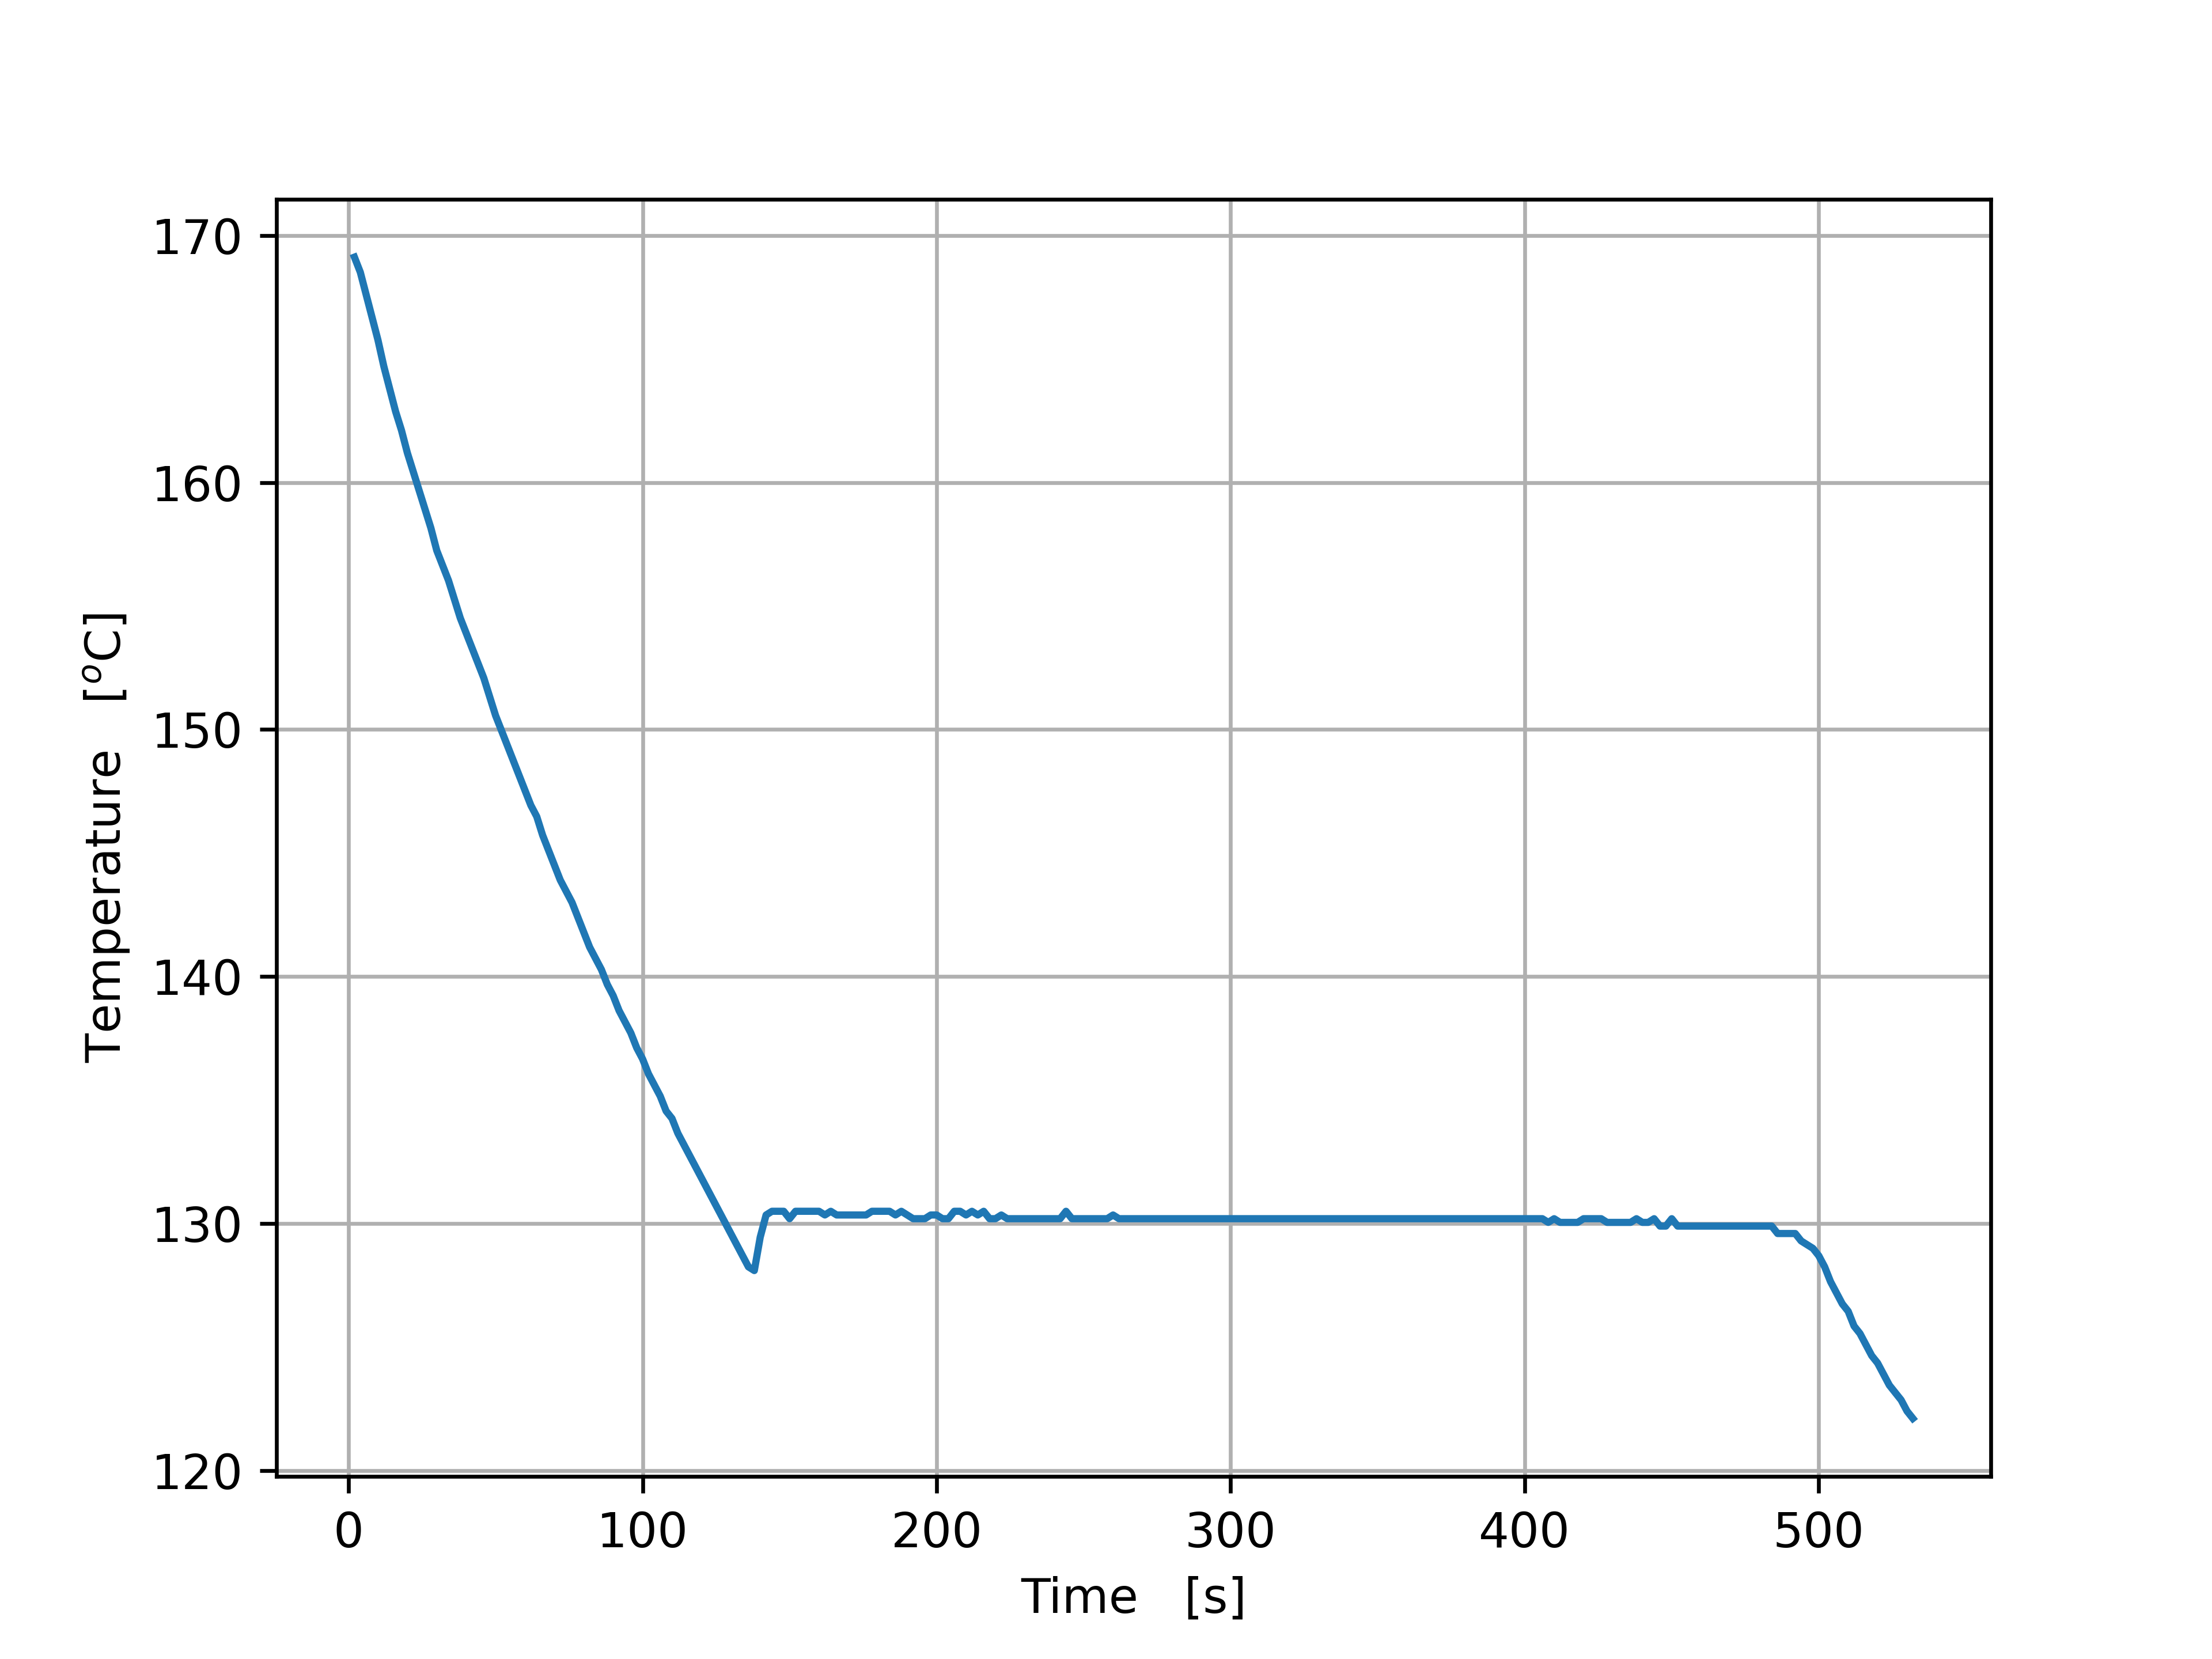
\includegraphics[width=0.5\linewidth]{plots/q1_00.png}
    \caption{Cooling Curve of Pure Tin}
    \label{fig:q1-00}
\end{figure}

\begin{figure}
    \centering
    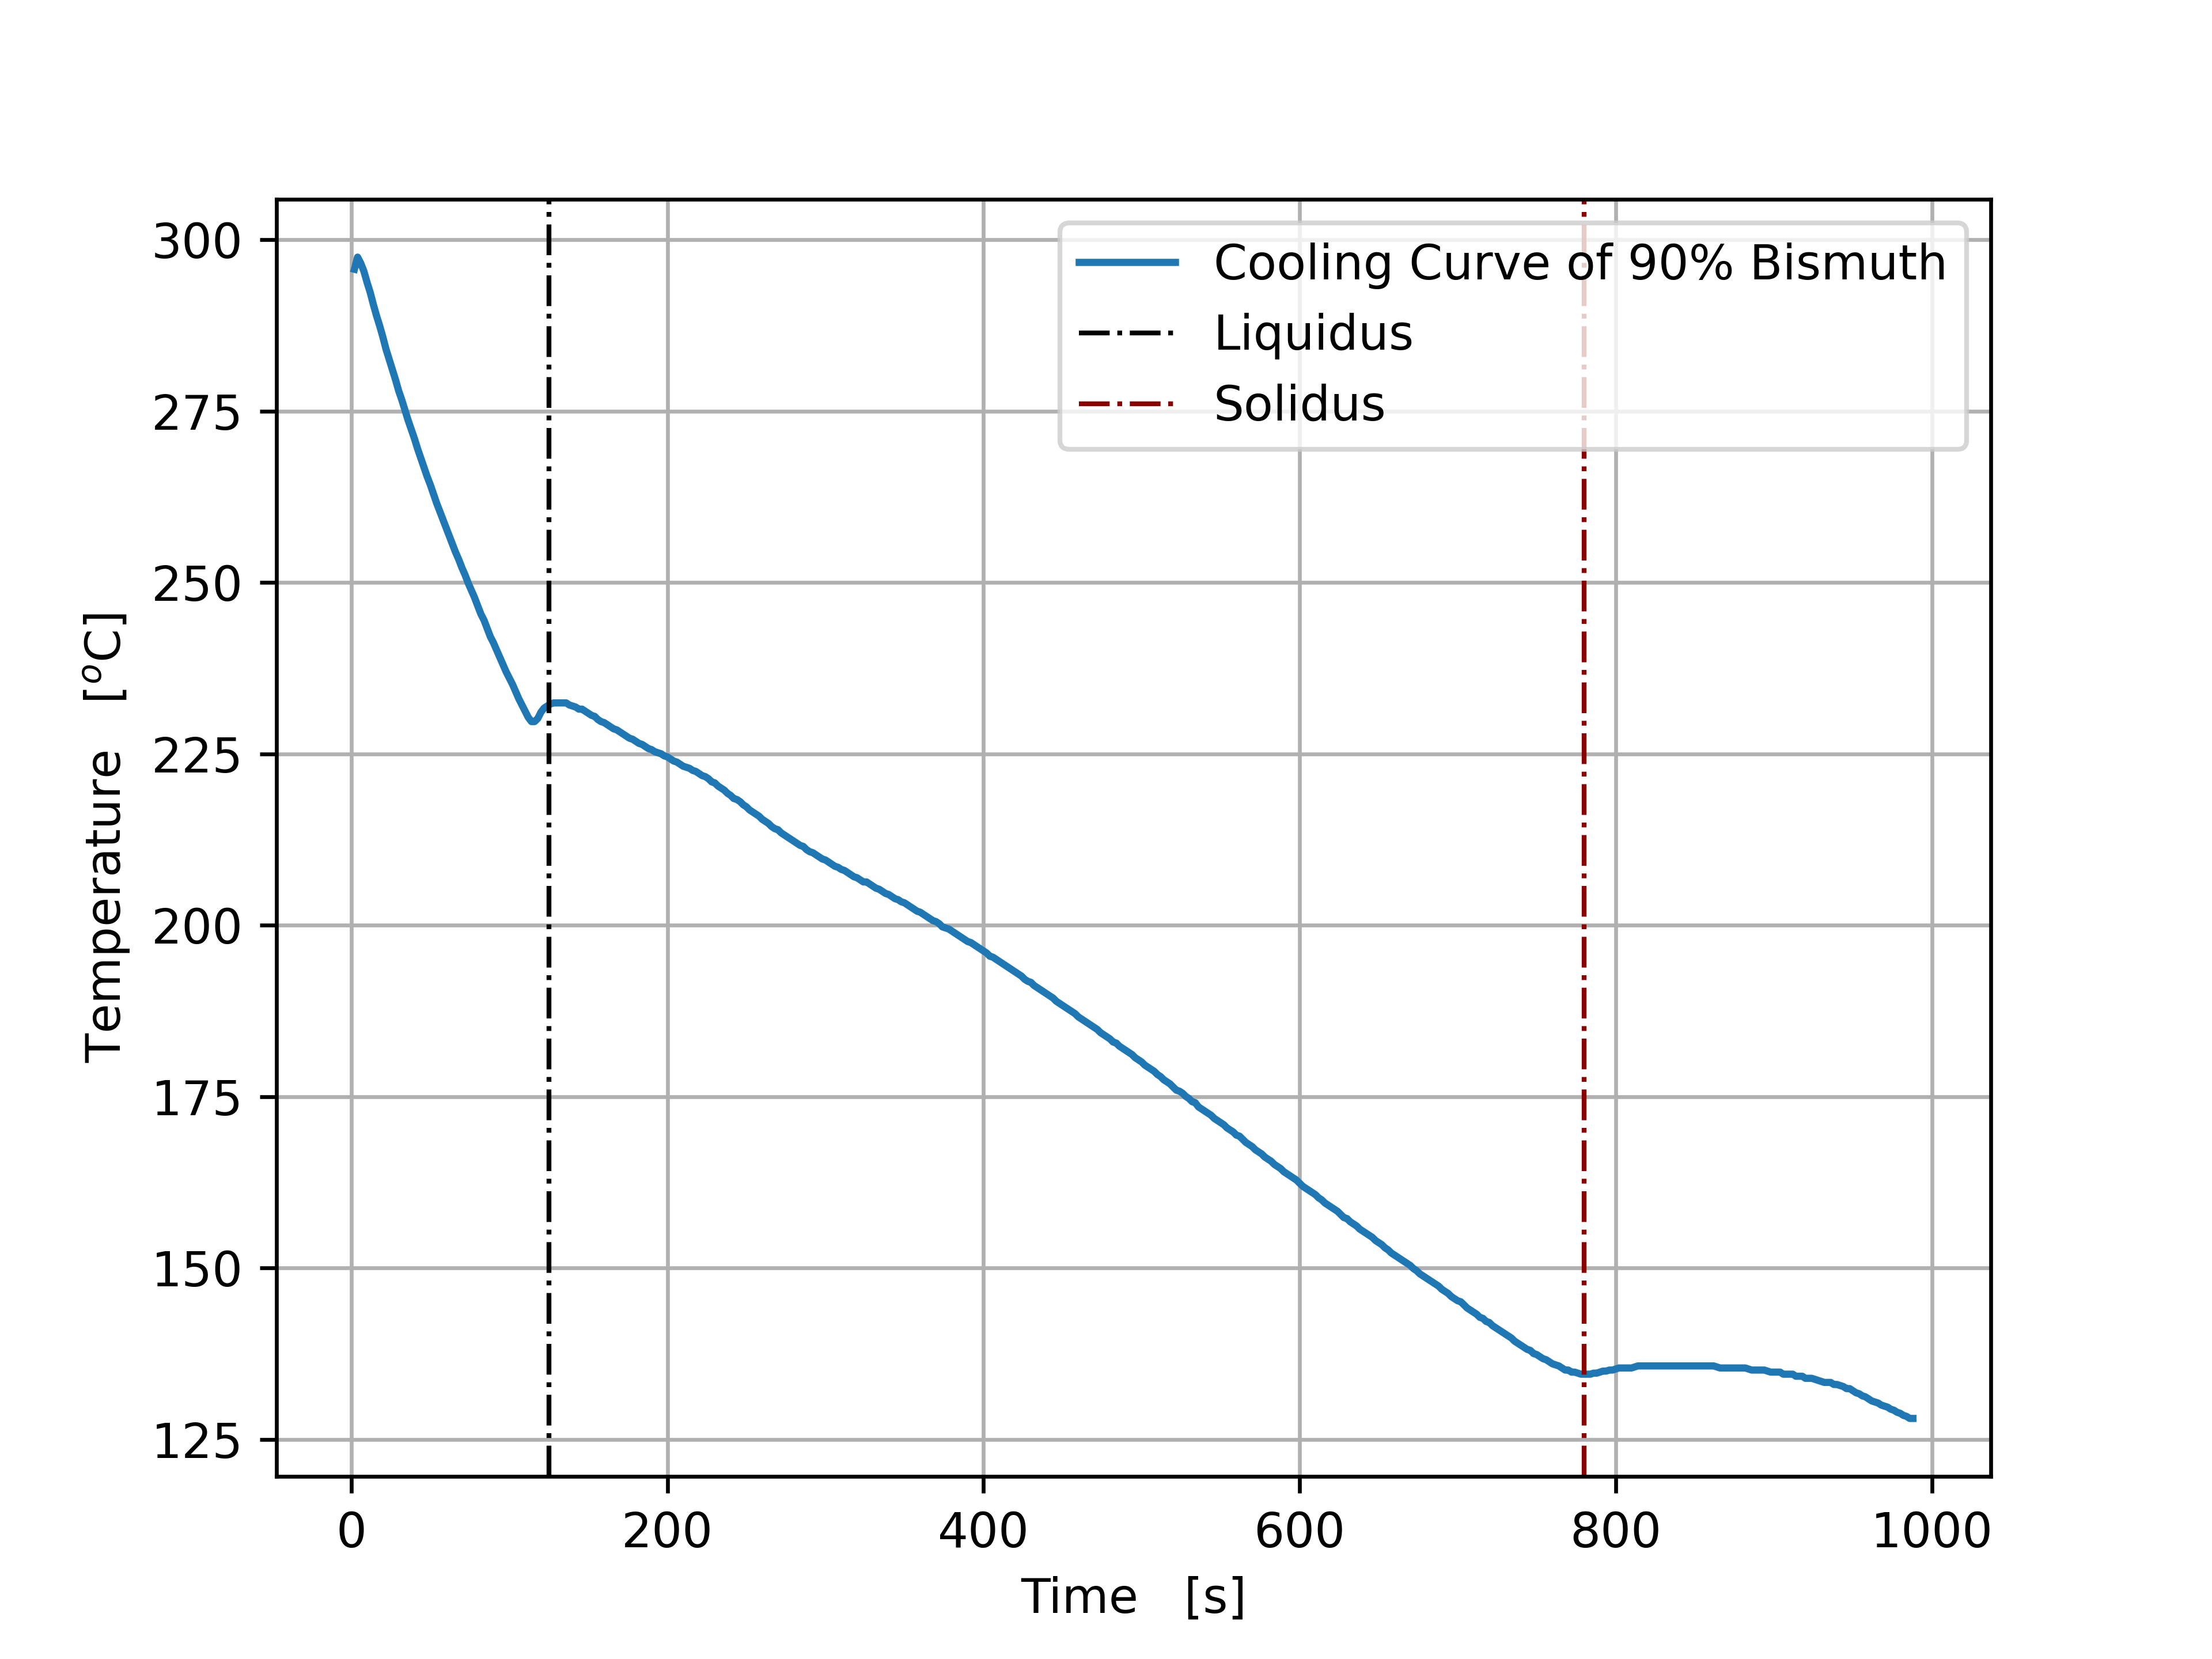
\includegraphics[width=0.5\linewidth]{plots/q1_90.png}
    \caption{Cooling Curve of 90\% Weight-Fraction Bismuth}
    \label{fig:q1-90}
\end{figure}

To continue, We plotted the cooling curves of pure tin, 25\% weight-fraction bismuth, 50\% weight-fraction bismuth, and 55\% weight-fraction bismuth. Alongside, we identified the micro-structure of each mixture. These are presented along-side each other for clarity. 

\begin{figure}
    \centering
    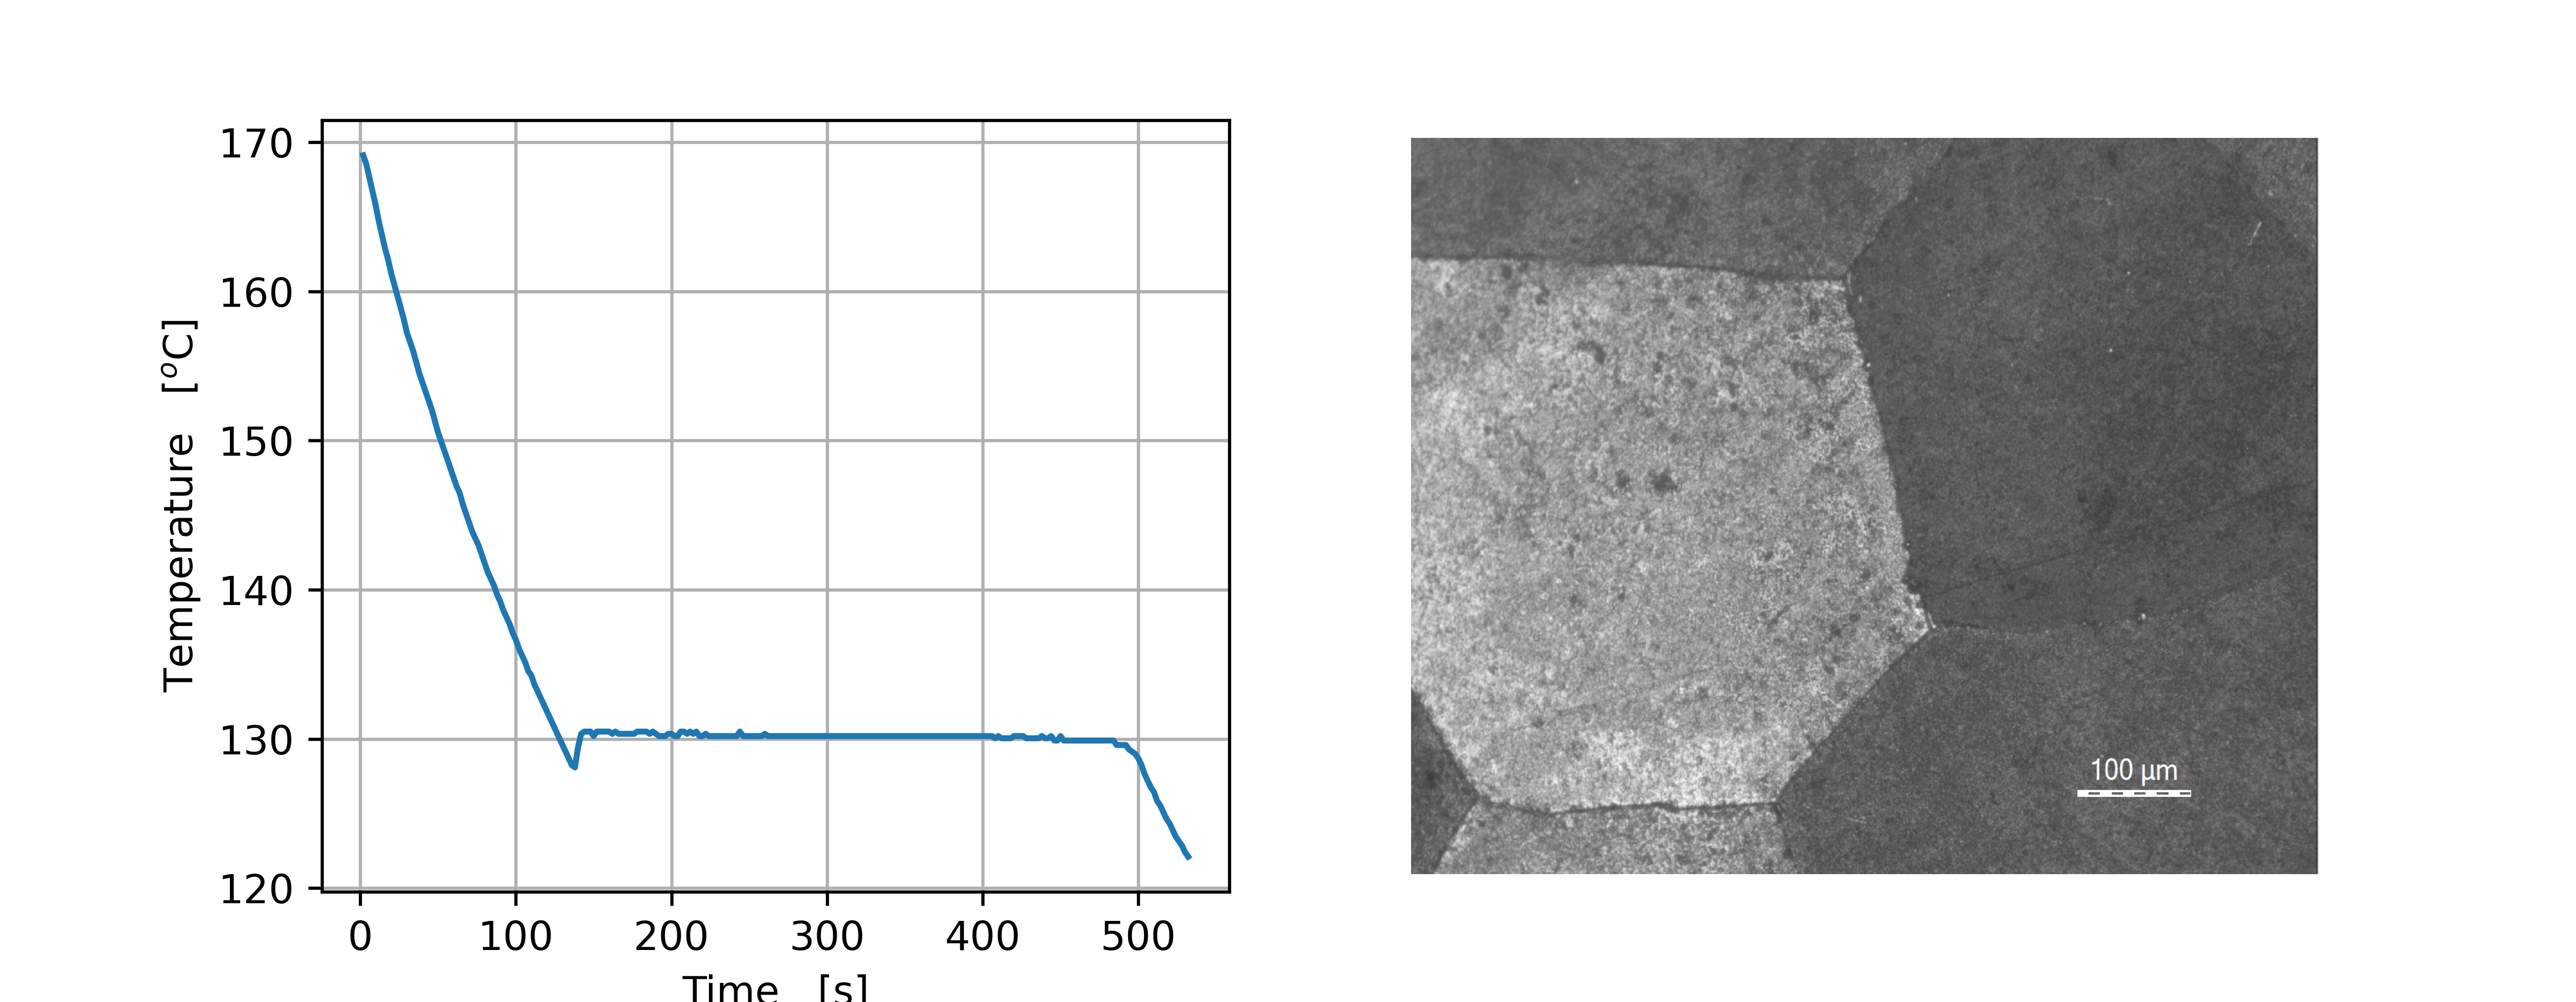
\includegraphics[width=1\linewidth]{plots/q2_00.png}
    \caption{Pure Tin cooling curve and micro-structure}
    \label{fig:q2-00}
\end{figure}

\begin{figure}
    \centering
    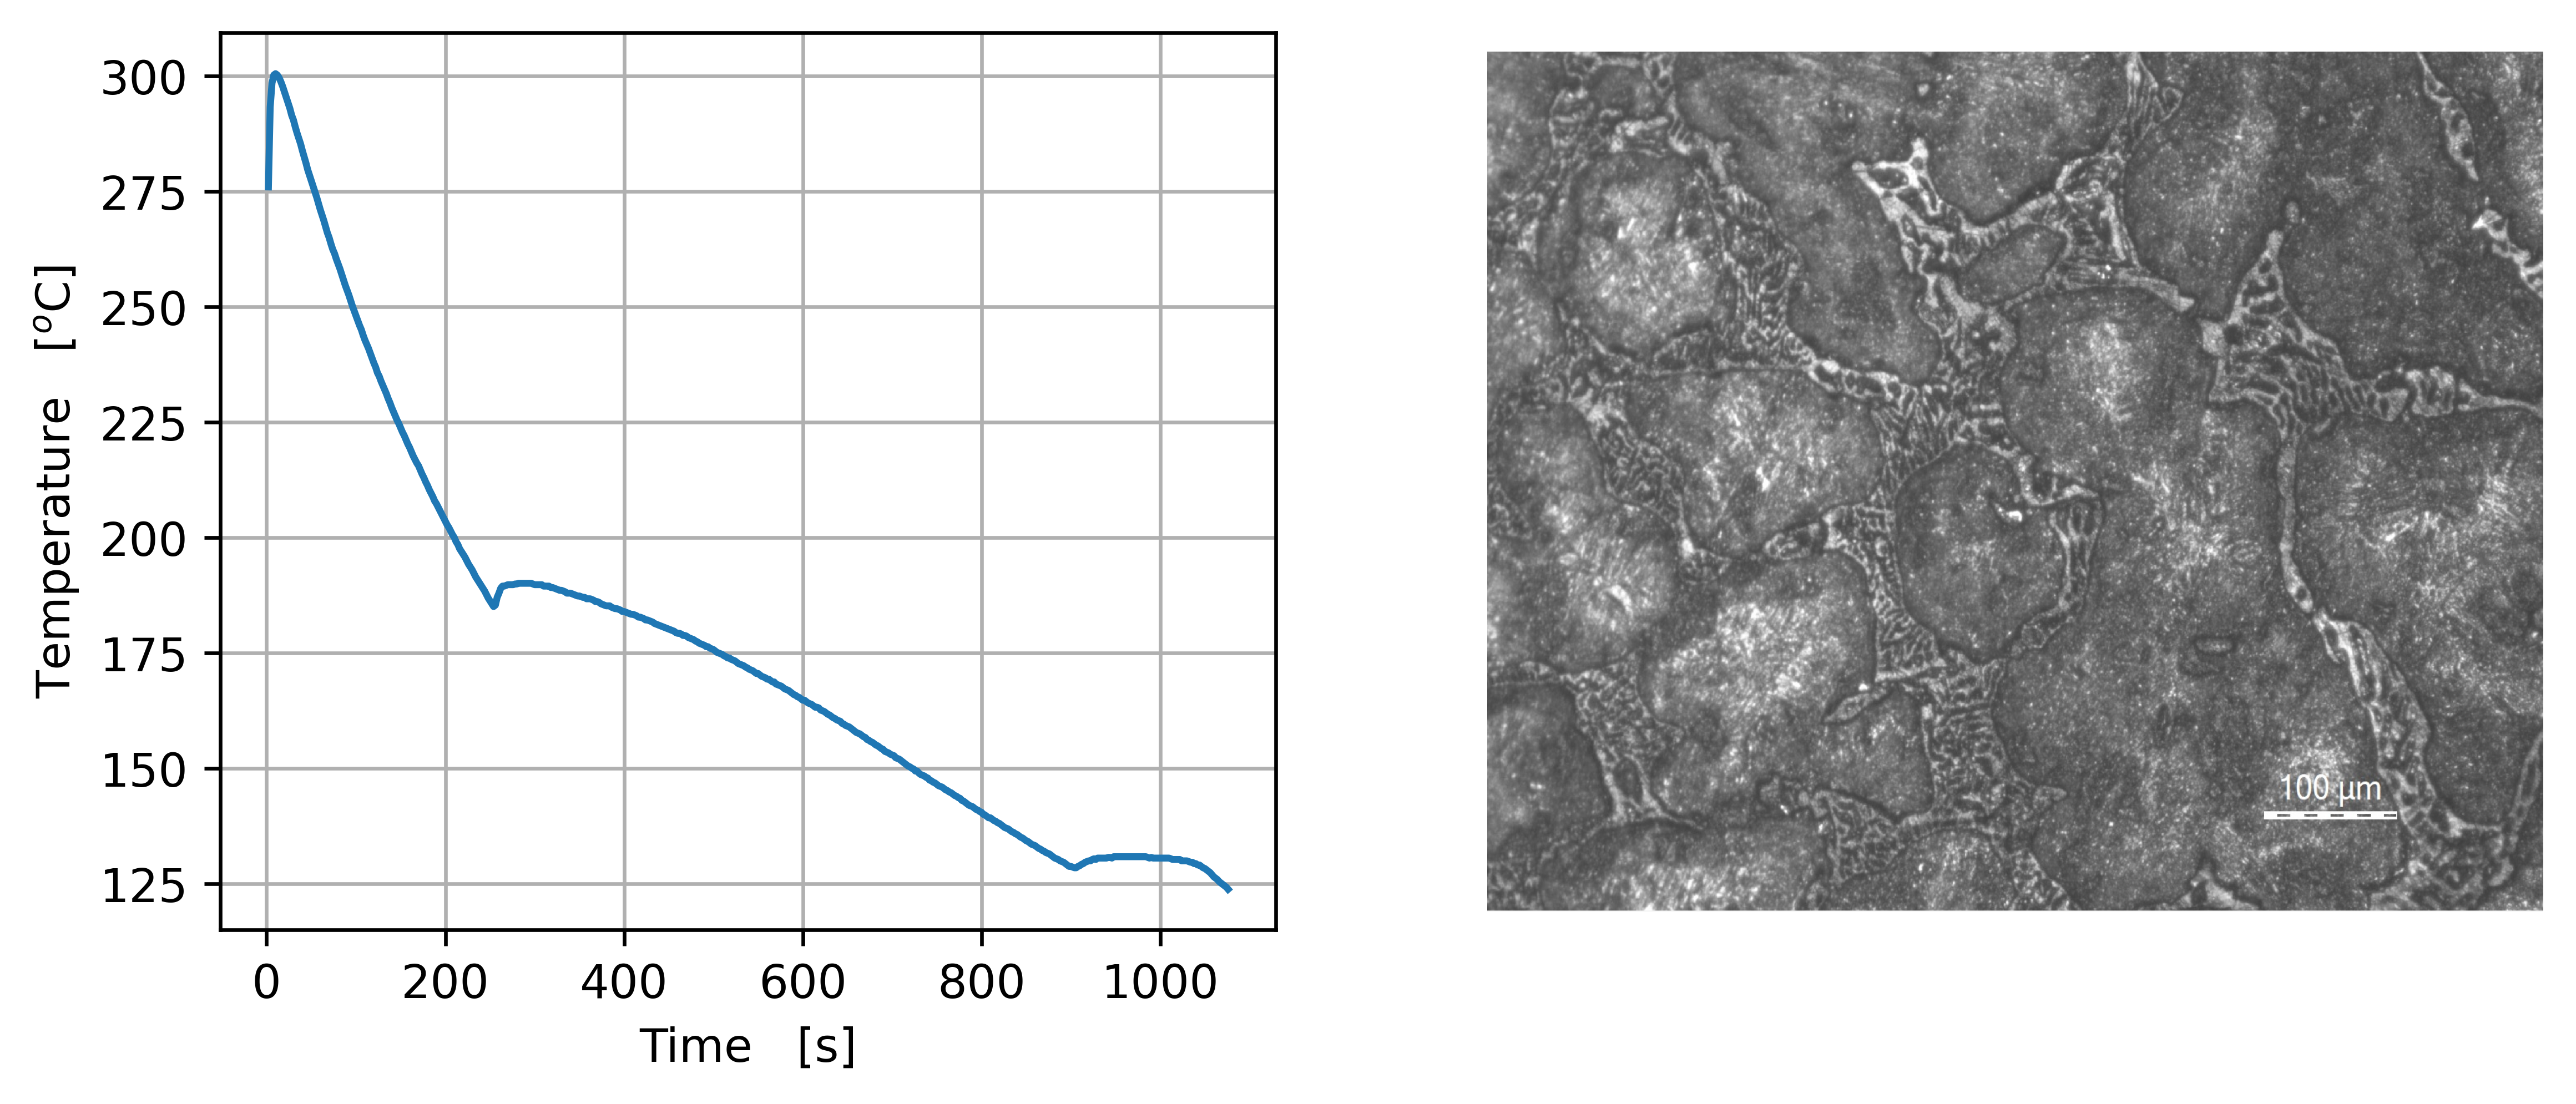
\includegraphics[width=1\linewidth]{plots/q2_25.png}
    \caption{25\% weight-fraction Bismuth cooling curve and micro-structure}
    \label{fig:q2-25}
\end{figure}

\begin{figure}
    \centering
    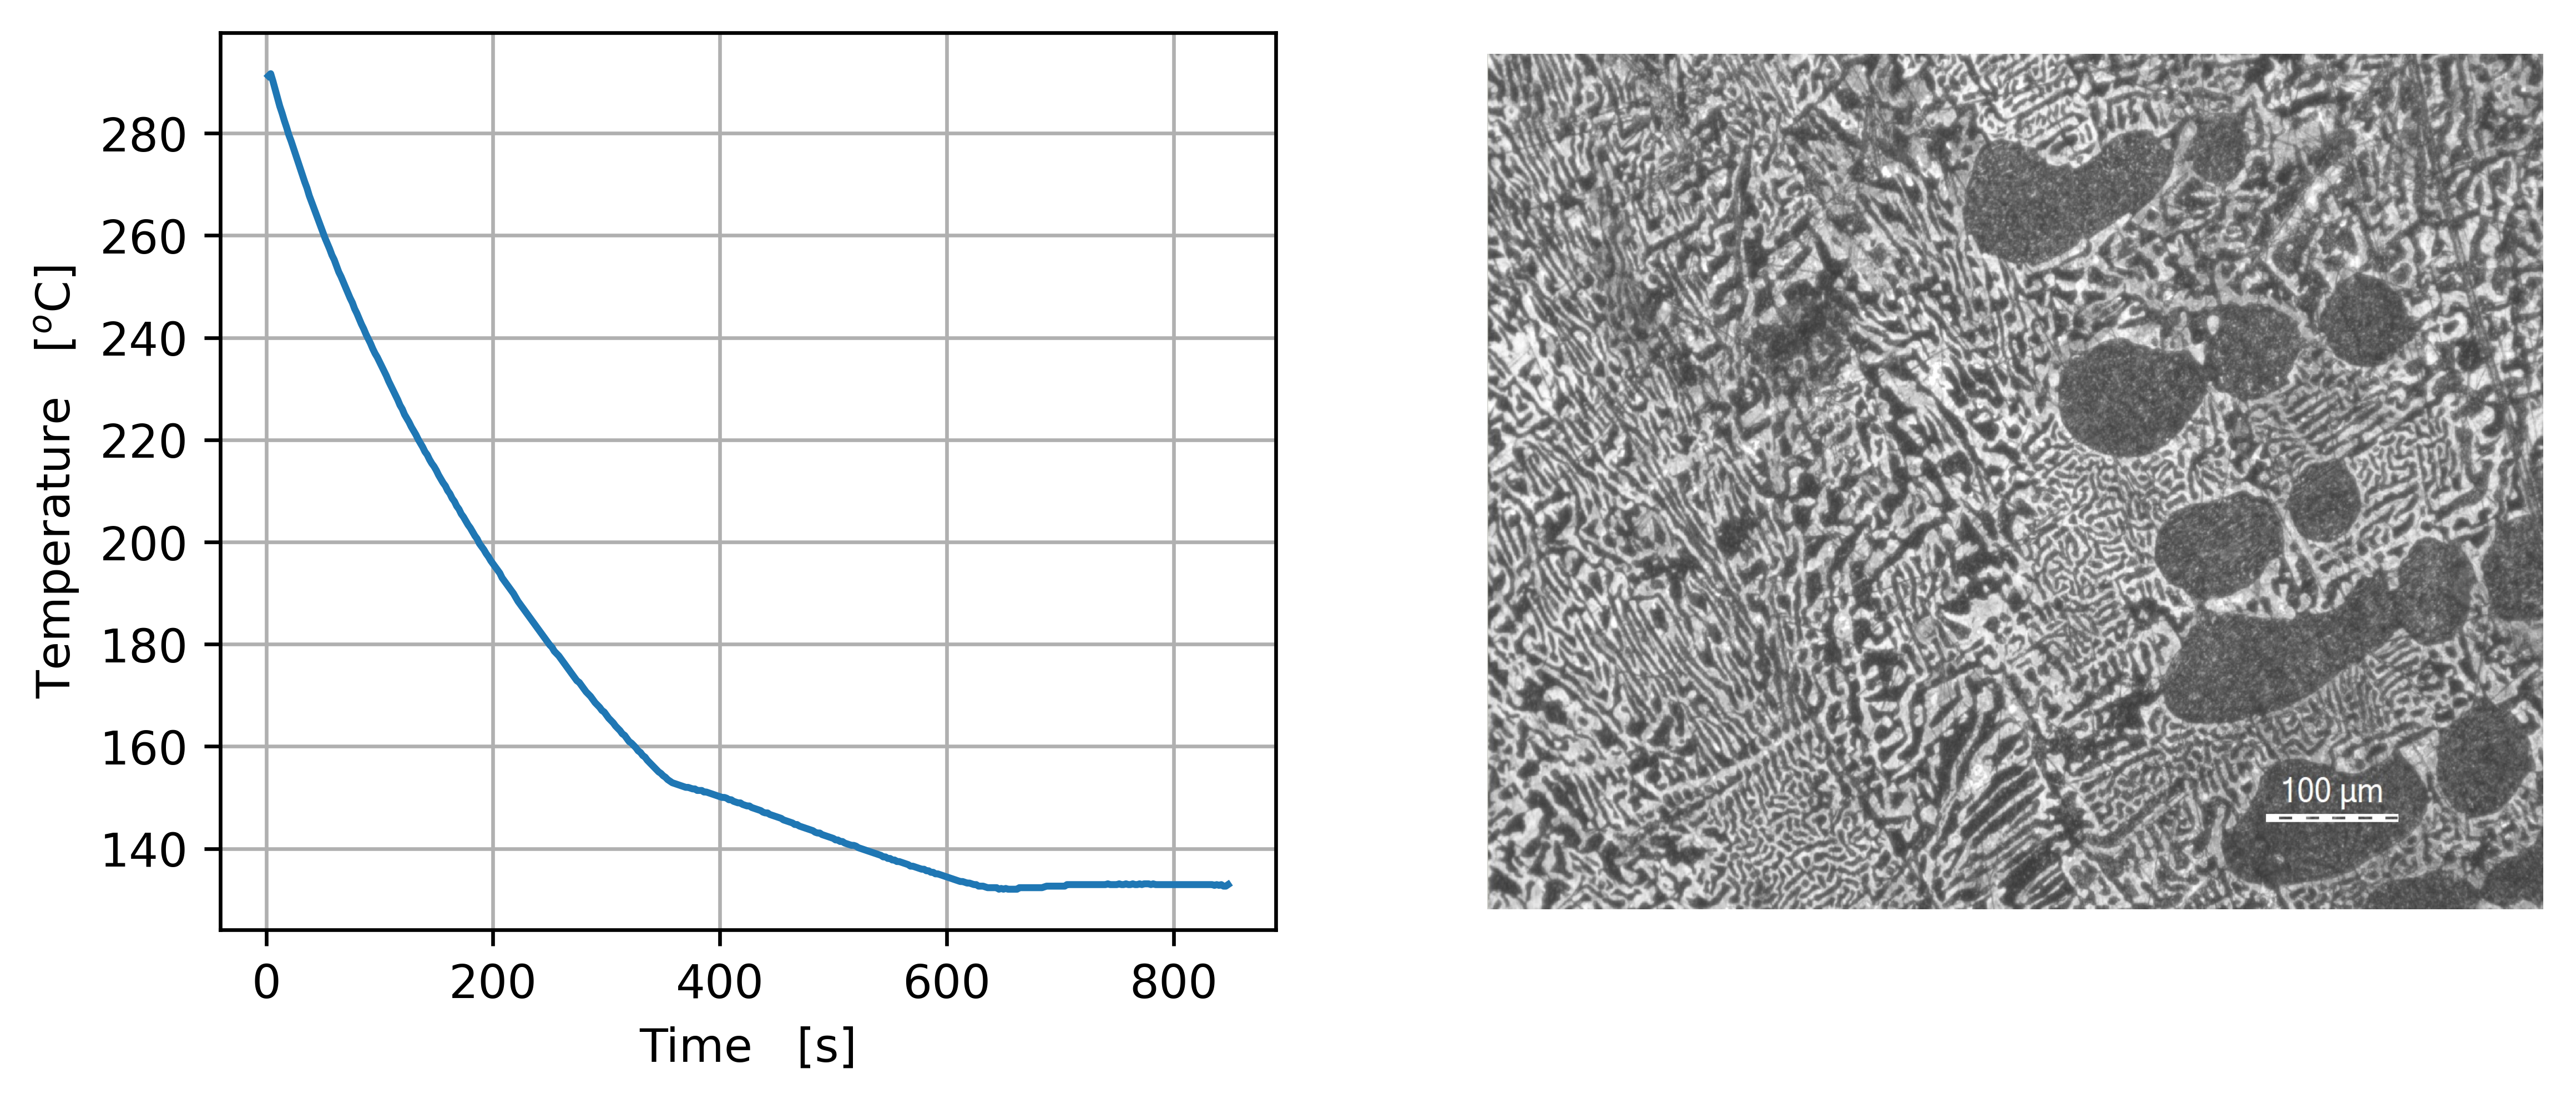
\includegraphics[width=1\linewidth]{plots/q2_50.png}
    \caption{50\% weight-fraction Bismuth cooling curve and micro-structure}
    \label{fig:q2-50}
\end{figure}

\begin{figure}
    \centering
    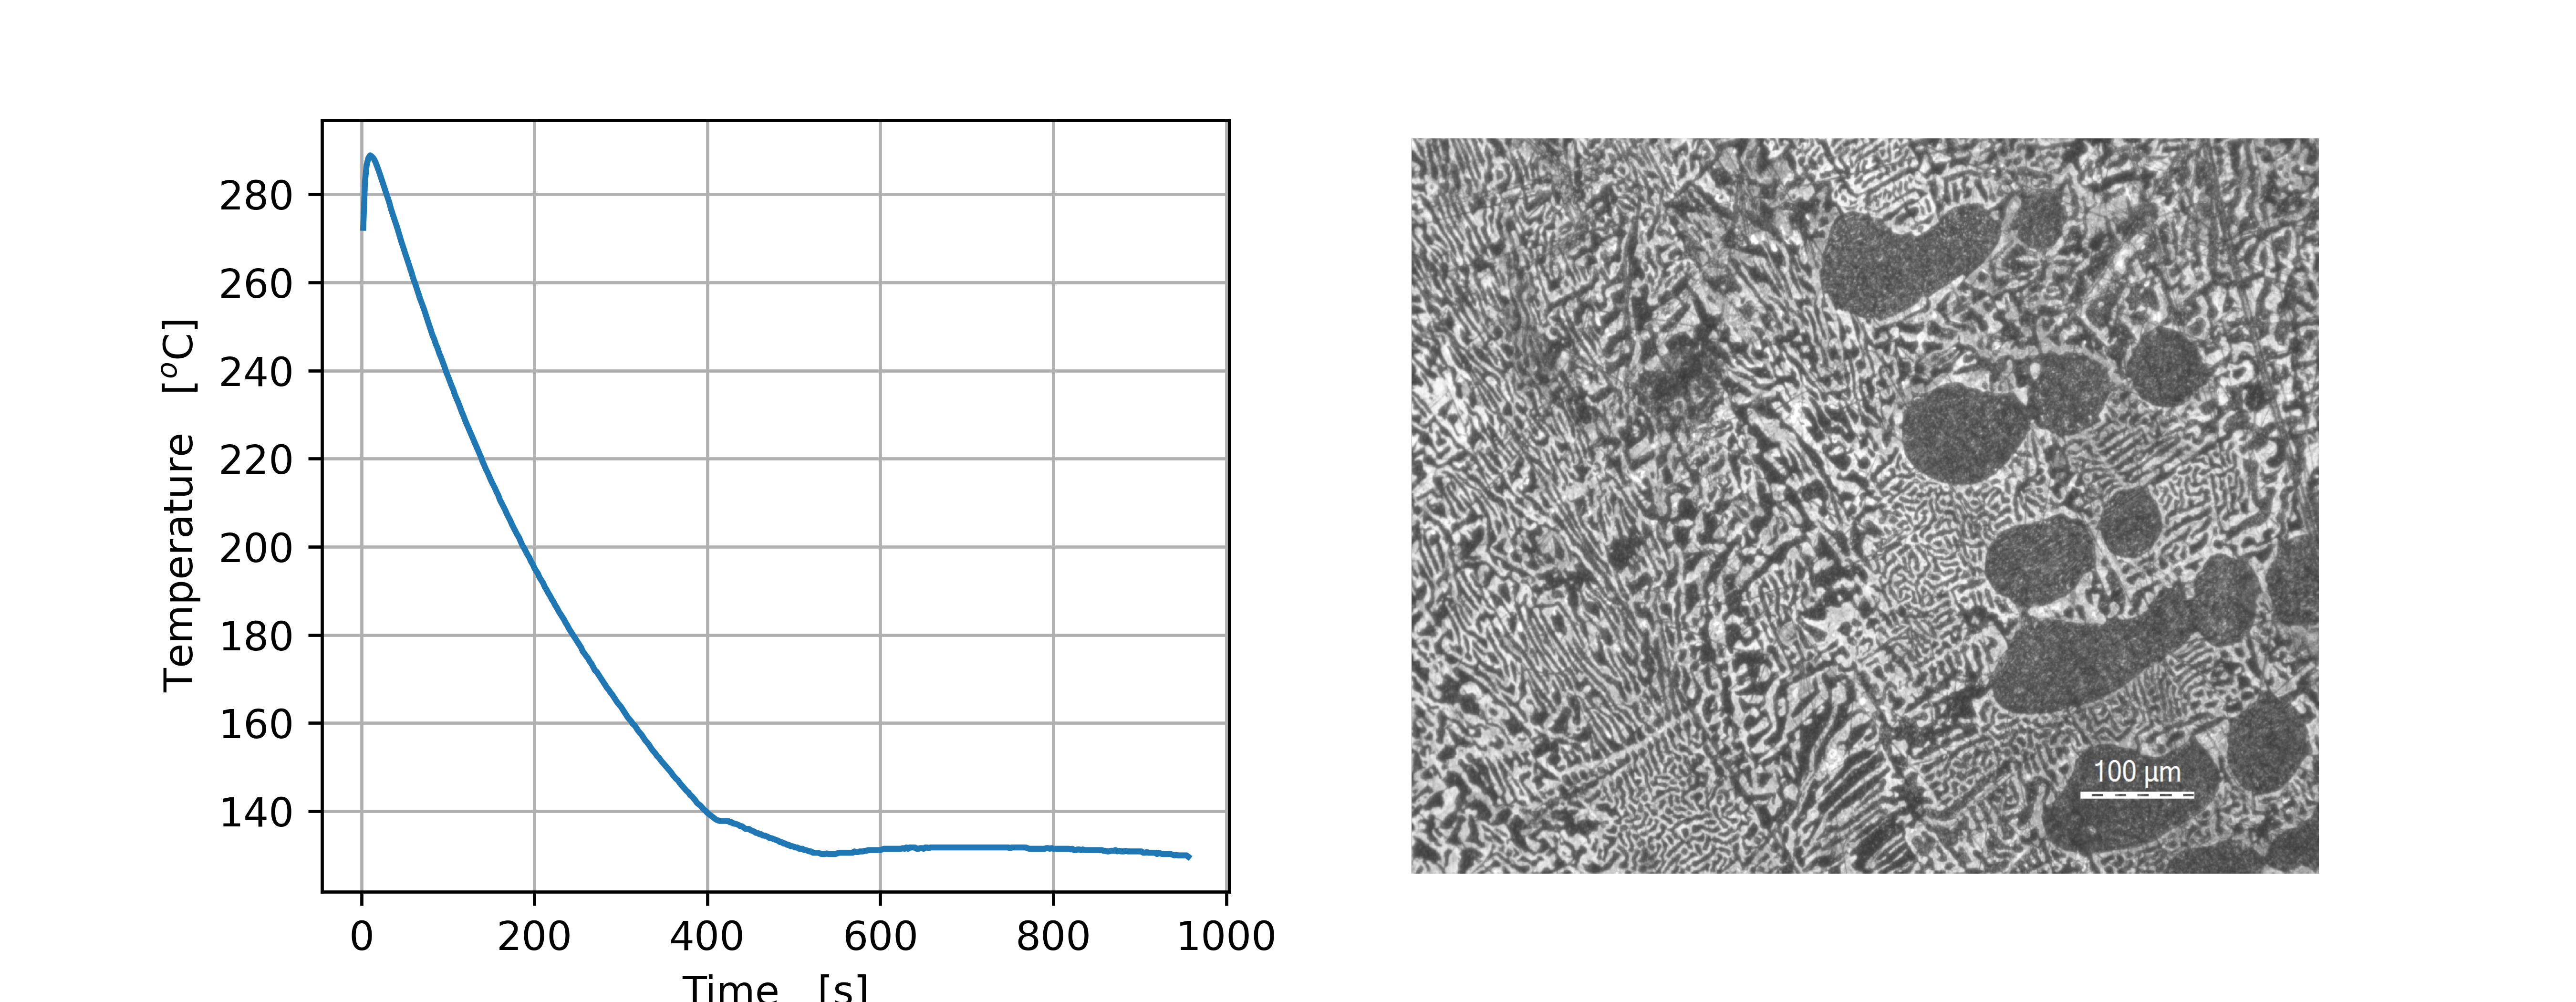
\includegraphics[width=1\linewidth]{plots/q2_55.png}
    \caption{55\% weight-fraction Bismuth cooling curve and micro-structure}
    \label{fig:q2-55}
\end{figure}




\section{Analysis and Discussion of Results}

\section{Answers to Questions}

\section{Conclusions}

\section{Bibliography}

\end{document}